\documentclass{article}

\usepackage{geometry}
\geometry{a4paper, margin=1in}
\usepackage{graphicx}
\usepackage{listings}
\usepackage{xcolor}
\usepackage[utf8]{inputenc}

\lstset{
    basicstyle=\ttfamily\small,
    breaklines=true,
    frame=single,
    language=C,
    keywordstyle=\color{blue},
    commentstyle=\color{green!50!black},
    stringstyle=\color{red}
}

\begin{document}

\title{Operating Systems Lab Assignment: Synchronization and Scheduling}
\author{Donovan Reed}
\date{October 2026}
\maketitle

\section{Introduction}

This report documents the implementation and analysis of synchronization and scheduling exercises using POSIX threads, mutexes, and condition variables. The programs demonstrate how synchronization prevents race conditions, controls execution order, avoids deadlocks, handles priority issues, and coordinates multiple threads safely.

% =========================================================
\section{Exercise 1: Hello World}

\lstinputlisting{hello_world.c}

\textbf{Explanation:}

The original program can fail if the shared variable and condition variable are not synchronized correctly. The child thread locks the mutex, increments \texttt{hello}, prints the first line, and signals the condition variable. The main thread waits inside a \texttt{while} loop until \texttt{hello} becomes 1 before printing the second line.

\textbf{Analysis:}

The mutex prevents both threads from modifying or checking \texttt{hello} at the same time. The condition variable allows the main thread to sleep until the child thread changes the shared state. The \texttt{while} loop is important because a condition variable wakeup does not guarantee that the condition is true until it is checked again.

\textbf{Screenshot:}

\begin{figure}[h]
    \centering
    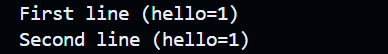
\includegraphics[width=\textwidth]{exercise1_screenshot.png}
    \caption{Compilation and execution of hello\_world.c}
\end{figure}

% =========================================================
\section{Exercise 2: SpaceX Problems}

\lstinputlisting{spacex.c}

\textbf{Explanation:}

The counter thread prints the values 3, 2, and 1 while protecting the shared variable \texttt{n} with a mutex. The announcer thread waits on the condition variable until the countdown reaches zero. It then prints ``FALCON HEAVY TOUCH DOWN!''.

\textbf{Analysis:}

Without synchronization, the announcer could inspect \texttt{n} at the wrong time and print before the countdown completes. The mutex protects the shared counter and the condition variable allows the announcer to wait efficiently. The \texttt{while} condition guarantees that the announcement occurs only after \texttt{n} reaches zero.

\textbf{Screenshot:}

\begin{figure}[h]
    \centering
    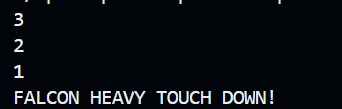
\includegraphics[width=\textwidth]{exercise2_screenshot.png}
    \caption{Compilation and execution of spacex.c}
\end{figure}

% =========================================================
\section{Exercise 3: I Love You, Unconditionally!}

\lstinputlisting{love.c}

\textbf{Explanation:}

The helper thread obtains the mutex and increments \texttt{subaru}. It then signals the condition variable. The main thread waits until \texttt{subaru} equals 1 before printing ``I love Emilia!''.

\textbf{Analysis:}

The solution follows Mesa semantics because the main thread checks the condition again after waking. The condition variable does not transfer execution directly to the waiting thread, so the shared condition must always be tested in a loop. The mutex also prevents a race condition on \texttt{subaru}.

\textbf{Screenshot:}

\begin{figure}[h]
    \centering
    
\includegraphics[width=\textwidth]{exercise3_screenshot.png}
    \caption{Compilation and execution of love.c}
\end{figure}

% =========================================================
\section{Exercise 4: Locking Up the Floopies}

\lstinputlisting{floopy.c}

\textbf{Explanation:}

The transfer operation must acquire two account locks. If two threads lock the same accounts in opposite orders, each thread could hold one lock while waiting for the other. This creates a circular wait and can cause deadlock. The corrected program always locks accounts in increasing UUID order.

\textbf{Analysis:}

For example, one thread may transfer from account 1 to account 2 while another transfers from account 2 to account 1. Without a consistent order, one thread could lock account 1 and the other could lock account 2. Both would then wait forever. Ordering the locks by UUID ensures that every thread requests the locks in the same sequence, eliminating circular wait.

\textbf{Screenshot:}

\begin{figure}[h]
    \centering
    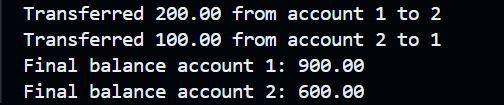
\includegraphics[width=\textwidth]{exercise4_screenshot.png}
    \caption{Compilation and execution of floopy.c}
\end{figure}

% =========================================================
\section{Exercise 5: Baking with Condition Variables}

\lstinputlisting{baking.c}

\textbf{Explanation:}

The baking program coordinates batter addition, egg addition, baking, and eating using a mutex and three condition variables. The batter and egg threads prepare the required ingredients. The heater waits until the bowl has enough batter and eggs, and the eater waits until the cake is ready.

\textbf{Analysis:}

The mutex protects the shared ingredient counts and the \texttt{readyToEat} flag. The \texttt{readyToBake} condition prevents baking from starting too early. The \texttt{startEating} condition prevents the eater from running before baking is complete. The \texttt{needIngredients} condition allows another baking cycle to begin only after the previous cake has been eaten.

\textbf{Screenshot:}

\begin{figure}[h]
    \centering
    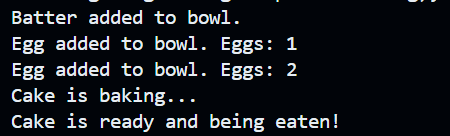
\includegraphics[width=\textwidth]{exercise5_screenshot.png}
    \caption{Compilation and execution of baking.c}
\end{figure}

% =========================================================
\section{Exercise 6: Priority Donation in Transfer}

\lstinputlisting{priority_transfer.c}

\textbf{Explanation:}

This program simulates priority donation using the custom priority field allowed by the assignment. When a higher-priority transfer uses an account that has a lower stored priority, the higher priority is temporarily assigned to the account state while the transfer is performed.

\textbf{Analysis:}

Priority inversion occurs when a high-priority thread must wait for a resource held by a lower-priority thread while another medium-priority thread continues running. Priority donation temporarily raises the effective priority associated with the required resource so that the blocking operation can complete sooner. In this implementation, donation is simulated with the custom priority field rather than modifying the Linux scheduler's actual thread priority.

\textbf{Screenshot:}

\begin{figure}[h]
    \centering
    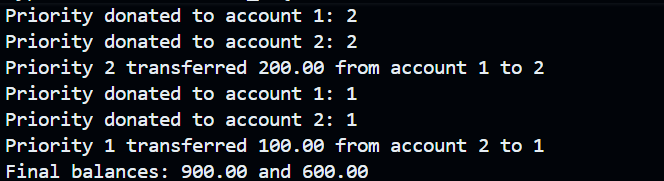
\includegraphics[width=\textwidth]{exercise6_screenshot.png}
    \caption{Compilation and execution of priority\_transfer.c}
\end{figure}

% =========================================================
\section{Exercise 7: Barrier Synchronization}

\lstinputlisting{barrier.c}

\textbf{Explanation:}

The barrier uses a mutex, condition variable, and shared counter. Each worker increments the counter when it reaches the barrier. Threads arriving before the final thread wait on the condition variable. When the final thread arrives, it broadcasts to wake all waiting threads.

\textbf{Analysis:}

The barrier ensures that no thread prints its ``After barrier'' message until every thread has reached the synchronization point. The mutex protects the shared counter, and the condition variable prevents waiting threads from continuing too early.

\textbf{Screenshot:}

\begin{figure}[h]
    \centering
    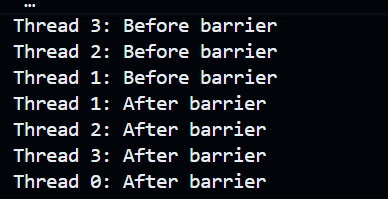
\includegraphics[width=\textwidth]{exercise7_screenshot.png}
    \caption{Compilation and execution of barrier.c}
\end{figure}

% =========================================================
\section{Exercise 8: Readers-Writers with Priority}

\lstinputlisting{readers_writers.c}

\textbf{Explanation:}

The program allows multiple readers to access shared data simultaneously while giving waiting writers priority. A reader waits whenever a writer is active or when \texttt{writer\_waiting} is greater than zero. A writer waits until no readers or other writer are active.

\textbf{Analysis:}

Writer priority is enforced by preventing new readers from entering once a writer begins waiting. Existing readers are allowed to finish, and then the writer receives access. After a writer completes, another waiting writer is signaled first. If no writers remain, all waiting readers are released.

\textbf{Screenshot:}

\begin{figure}[h]
    \centering
    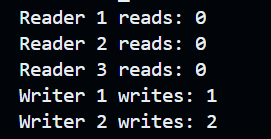
\includegraphics[width=\textwidth]{exercise8_screenshot.png}
    \caption{Compilation and execution of readers\_writers.c}
\end{figure}

% =========================================================
\section{Exercise 9: Thread Pool}

\lstinputlisting{thread_pool.c}

\textbf{Explanation:}

The thread pool creates a fixed number of worker threads and stores tasks inside a thread-safe queue. Workers wait for tasks using a condition variable and remove available tasks from the queue. The mutex protects the queue's head, tail, count, and shutdown state.

\textbf{Analysis:}

A thread pool is more efficient than creating a new thread for every task because the worker threads are created once and reused. This reduces repeated thread creation and destruction overhead. The \texttt{not\_empty} and \texttt{not\_full} condition variables coordinate producers and workers while preventing race conditions in the queue.

\textbf{Screenshot:}

\begin{figure}[h]
    \centering
    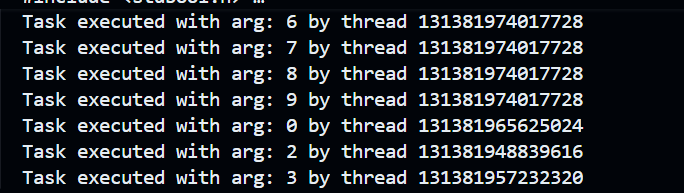
\includegraphics[width=\textwidth]{exercise9_screenshot.png}
    \caption{Compilation and execution of thread\_pool.c}
\end{figure}

% =========================================================
\section{Conclusion}

These exercises demonstrate how POSIX synchronization mechanisms can coordinate concurrent programs safely. Mutexes provide mutual exclusion for shared state, while condition variables allow threads to wait for specific conditions without continuously polling. Consistent lock ordering prevents deadlocks, writer-priority rules control access order, barriers synchronize groups of threads, and thread pools efficiently reuse worker threads.

\end{document}
